\subsubsection{Consensus} \label{odp_consensus}
% Subsection structure:
% Problem: what is the generalized problem?
% 	Motivation: why is this problem scientifically important and/or interesting?
% Solution: conceptual description of solution, including formal definition of GODP and SHACL shapes.
% 	Illustration: images of GODP structure.
% 	(Statistical)Analysis: how does the solution solve the problem?
% 	Evaluation: are the results significant? What is the impact?
\paragraph{Detecting consensus}
Information that is based on multiple evidence sources is more reliable than information that is based on one evidence source. For example, one scientific paper supported by stakeholder experience is more reliable than a scientific paper alone. 

\begin{center}
\large\color{document}{The consensus pattern validates the evidence reliability by detecting when evidence does not agree with at least one additional evidence source.}
\end{center}

\paragraph{Ontology}
We define consent evidence as evidence that agrees with at least one other evidence source. The reproducibility pattern provides the structure on which we create the consensus pattern. We introduce the $agrees\_with$ object property. Figure \ref{fig:consensus} presents the consensus pattern. We mark the extension of the reproducibility pattern in \textcolor{LightGreen}{green}. For example, if two stakeholders have the same experience, the $agrees\_with$ object property can link this stakeholder experience. 

\begin{figure}[H]
\centering
  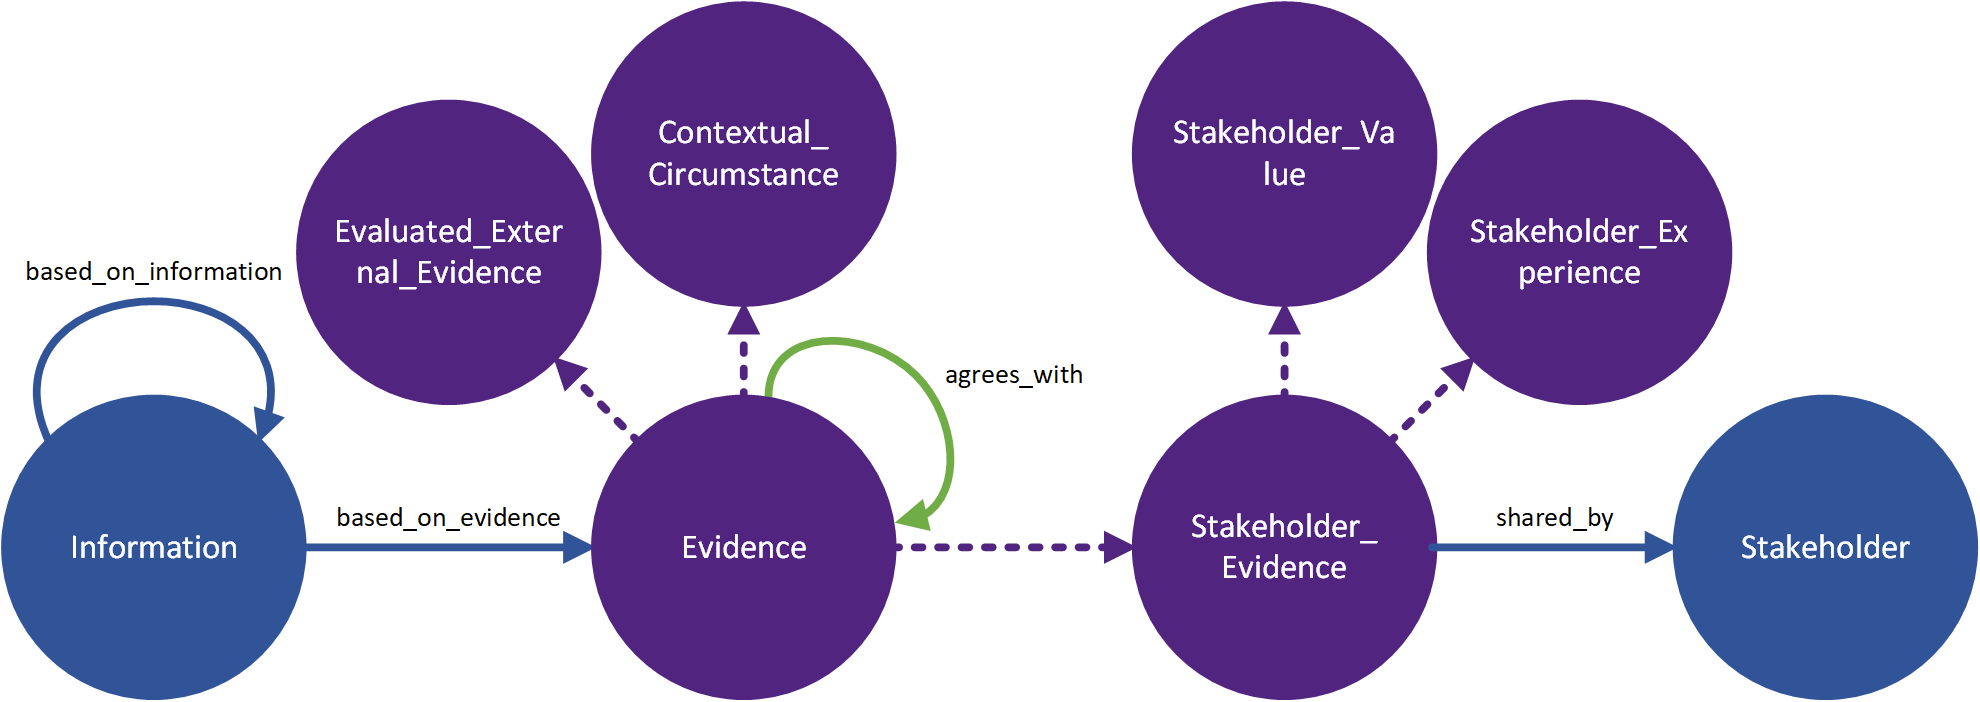
\includegraphics[width=14cm]{../../Images/04_Contribution/04_Consensus_Ontology.png}
  \caption{The consensus pattern that we have based on the reproducibility pattern. We have extended the reproducibility pattern with the object property $agrees\_with$. Code sample \ref{GODP_CON_LEV} extends the reproducibility pattern using GDOL.}
  \label{fig:consensus}
\end{figure}

\paragraph{Inferencing}
We can measure the consensus-level of an evidence source using the $agrees\_with$ object property. We extend the $based\_on\_evidence$ object property with a super property. When we base $In{\f}ormationX$ on $EvidenceA$, and $EvidenceA$ agrees with $EvidenceB$, the reasoner bases $In{\f}ormationX$ on $EvidenceB$ as well. Figure \ref{fig:consensus_inferred} presents the super property that infers this knowledge from the existing ontology structure.

\begin{figure}[H]
\centering
  
\includegraphics[width=17cm]{../../Images/Consensus_Inferred.png}
  \caption{The super property that infers the object property $based\_on\_evidence$ in Prot\'eg\'e.}
  \label{fig:consensus_inferred}
\end{figure}

The $agrees\_with$ object property is symmetric. If individual $A$ agrees with individual $B$, individual $B$ should also agree with individual $A$. Figure \ref{fig:consensus_transitive} presents the characteristics of the $agrees\_with$ object property.

\begin{figure}[H]
\centering
  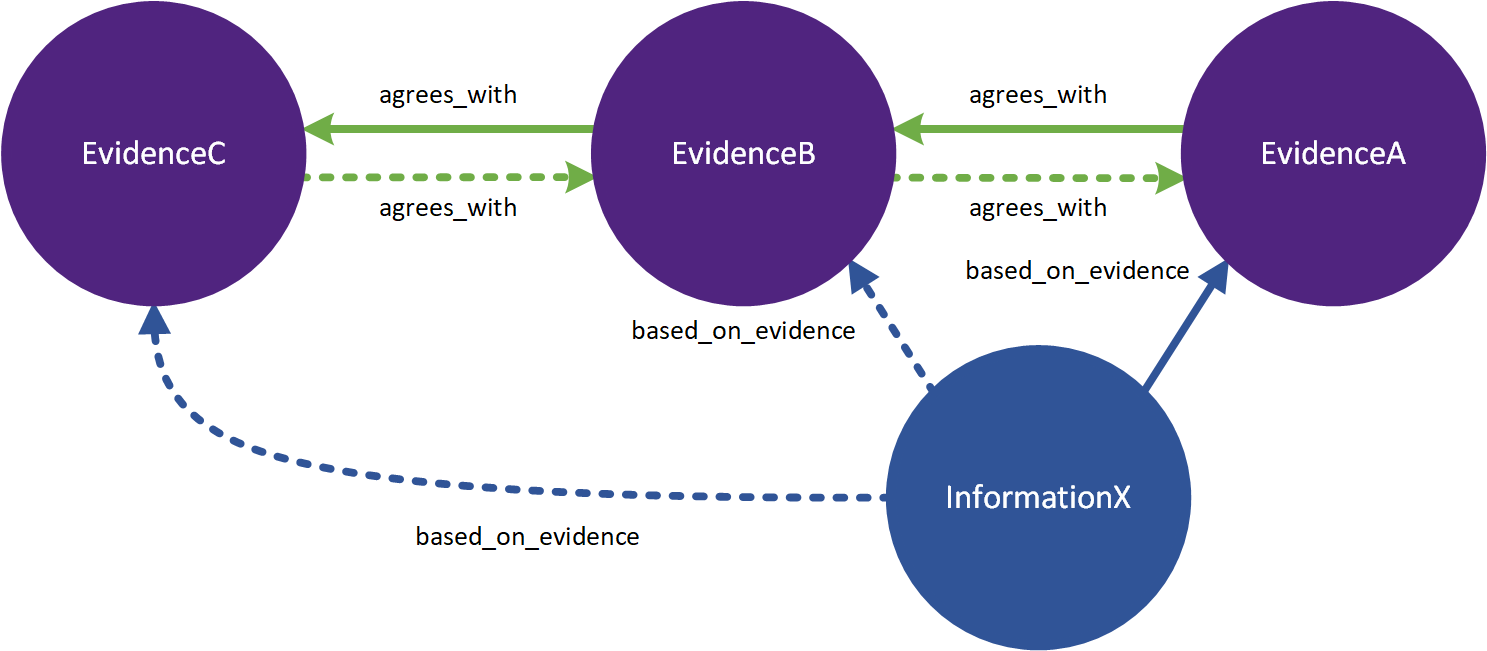
\includegraphics[width=13cm]{../../Images/04_Contribution/04_Consensus_Characteristics.png}
  \caption{An example of the impact of the symmetric characteristics of the $agrees\_with$ object property. The reasoner infers the dotted lines based on the super property figure \ref{fig:consensus_inferred} presents and the symmetric characteristics of $agrees\_with$.}
  \label{fig:consensus_transitive}
\end{figure}

\paragraph{Inconsistency}
The consensus pattern inherits the consistency validation from the reproducibility pattern. We describe the consistency of the reproducibility pattern in section \ref{rep_incons} \nameref{rep_incons}.

\paragraph{Generic ontology design pattern}
Code sample \ref{GODP_CON_LEV} presents the described solution into GDOL. We take the $Reproducibility\_Basic$ pattern, introduce the $agrees\_with$ object property, and extend the $based\_on\_evidence$ object property. 

\begin{lstlisting}[float,language=GDOL,caption={The GDOL code that extends the reproducibility pattern and results in the consensus pattern. We take the $Reproducibility\_Basic$ pattern, introduce the $agrees\_with$ object property, and extend the $based\_on\_evidence$ object property. Figure \ref{fig:consensus} presents the generic ontology design pattern.},label={GODP_CON_LEV}][H]
ontology Consensus = Reproducibility_Basic then
 ObjectProperty: agrees_with Domain: Evidence Range: Evidence Characteristics: Symmetric
 ObjectProperty: based_on_evidence SubPropertyChain: based_on_evidence o agrees_with SubPropertyOf: based_on_evidence
\end{lstlisting}

\paragraph{Constraints}
We define one consensus level for each individual classified as $Evidence$. We set the consensus-level to $1$. This consensus level ensures that each used evidence source has at least one other agreeable evidence source. The minimum consensus level can be adjusted depending on the environment. For example, in life-safety environments, the consensus level might be increased. We use the cardinality constraint $sh:minCount$ for the consensus detection: each individual classified as $Evidence$ should have at least one path $agrees\_with$.

\begin{lstlisting}[float,language=SHACL,caption={The SHACL shapes that detect when information does not meet the minimum consensus level.},label={SHACL_CON_LEV}][H]
UsedEvidenceShape a sh:NodeShape;
	sh:targetClass Evidence; 
	sh:property [
		sh:path agrees_with; 
		sh:severity sh:Violation; 
		sh:minCount 1; 
		sh:message "Consensus: ensure the evidence is in agreement with at least one additional evidence source."; ];
\end{lstlisting}